% ---
% Inserir folha de aprovação
% ---

% Isto é um exemplo de Folha de aprovação, elemento obrigatório da NBR
% 14724/2011 (seção 4.2.1.3). Você pode utilizar este modelo até a aprovação
% do trabalho. Após isso, substitua todo o conteúdo deste arquivo por uma
% imagem da página assinada pela banca com o comando abaixo:
%
% \includepdf{folhadeaprovacao_final.pdf}
%
%\begin{folhadeaprovacao}
%	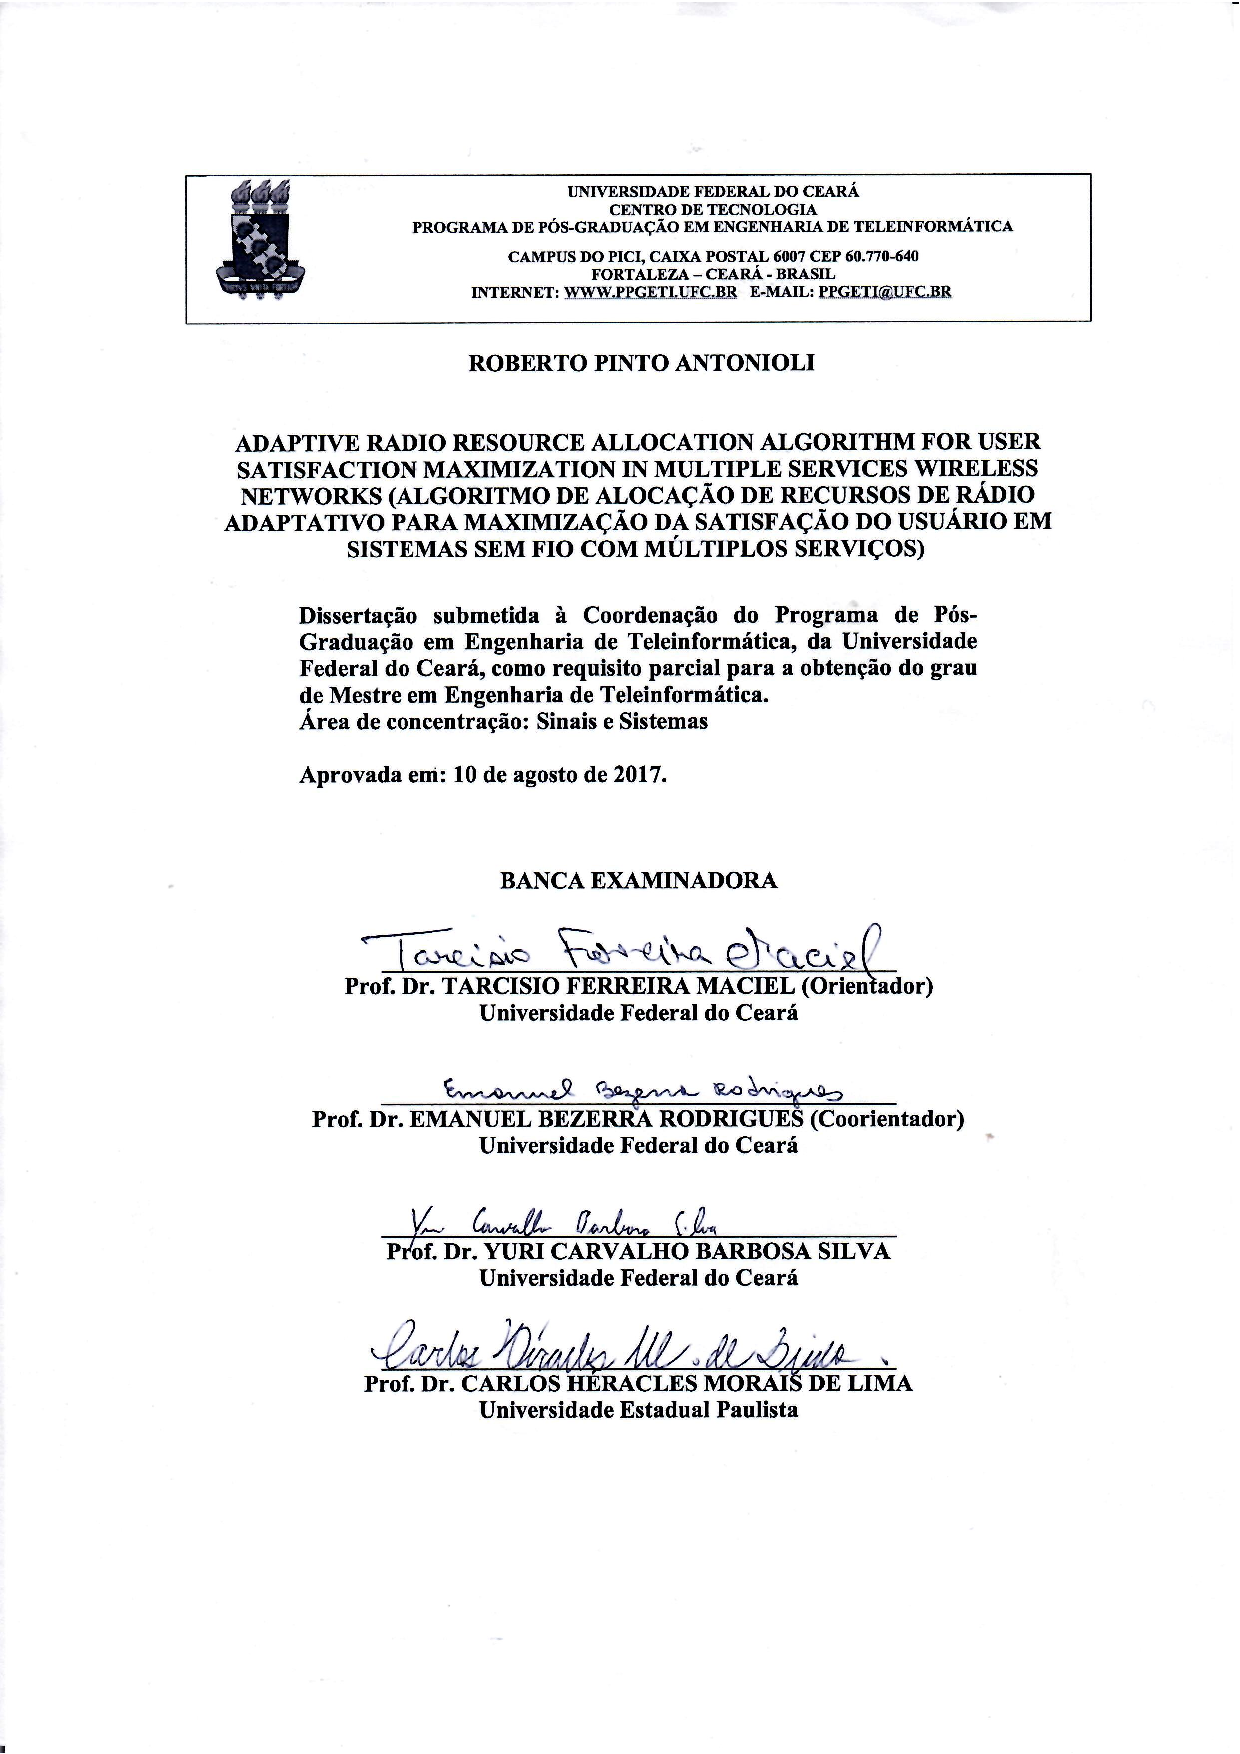
\includepdf{editaveis/aprovacao.pdf}
%\end{folhadeaprovacao}
% ---

% ---
% Inserir folha de aprovação
% ---

% Isto é um exemplo de Folha de aprovação, elemento obrigatório da NBR
% 14724/2011 (seção 4.2.1.3). Você pode utilizar este modelo até a aprovação
% do trabalho. Após isso, substitua todo o conteúdo deste arquivo por uma
% imagem da página assinada pela banca com o comando abaixo:
%
% \includepdf{folhadeaprovacao_final.pdf}
%
\begin{folhadeaprovacao}
	
	\begin{center}
		{\MakeUppercase\imprimirautor}
		\vspace{1cm}
		
		\begin{center}
			\MakeUppercase\imprimirtitulo
		\end{center}
		
		\vspace{2cm}
		\hspace{.45\textwidth}
		\begin{minipage}{0.5\textwidth}
			Monografia apresentada ao Curso de Engenharia de Computação da Universidade Federal do Ceará, como parte dos requisitos para obtenção do Título de Bacharel em Engenharia de Computação.
			\\ \\ \\
		\end{minipage}
		
		\vspace{-0.5cm}
		
		\begin{minipage}{\textwidth}
			Aprovada em: 18/12/2017.
		\end{minipage}
		
		\vspace{0.5cm}
		BANCA EXAMINADORA
	\end{center}
	
	\def\spacebetweensigns{-12pt}
	
	\vspace{\spacebetweensigns}
	\assinatura{}
	\vspace{\spacebetweensigns}
	\begin{center}
		{\imprimirorientador \space (Orientador) \\ Universidade Federal do Ceará (UFC)}
	\end{center}
	
	%DEFINA AQUI OS DEMAIS MEMBROS DA BANCA
	
	\vspace{\spacebetweensigns}
	\assinatura{}
	\vspace{\spacebetweensigns}
	\begin{center}
		{Prof. Msc. Marcelo Araújo Lima  \space (Co-Orientador) \\ Instituto Federal do Ceará (IFCE)}
	\end{center}
	
	\vspace{\spacebetweensigns}
	\assinatura{}
	\vspace{\spacebetweensigns}
	\begin{center}
		{Prof. Dr. Jarbas Aryel da Silveira \\ Universidade Federal do Ceará (UFC)}
	\end{center}
	
	\vspace{\spacebetweensigns}
	\assinatura{}
	\vspace{\spacebetweensigns}
	\begin{center}
		{Prof. Msc. Daniel Alencar Barros Tavares \\ Instituto Federal do Ceará (IFCE)}
	\end{center}
		
\end{folhadeaprovacao}
% ---